\chapter{Regression}
\label{chap:regression}

%%%%%%%%%%%%%%%%%%%%%%%%%%%%%%%%%%%%%%%%%%%%%%%%%%%%%%%%
% \section{Linear Regression}
% \label{regression:linear}
% TODO

%%%%%%%%%%%%%%%%%%%%%%%%%%%%%%%%%%%%%%%%%%%%%%%%%%%%%%%%
\section{Logistic Regression}
\label{regression:logistic}

Logistic regression is a simple method to create a classifier,
typically on two classes $y = 0,1$, though multinomial extensions exist.
Its name comes from the use of the logit, or log-odds, function

\begin{equation}\label{eq:logistic:logic}
l = \text{logit}\left(p\right) = \log\left(\frac{p}{1-p}\right)
\end{equation}

\noindent on the probability $p$ of class $1$.
$l$ is estimated linearly from $m$ input features $x_{i}$ with $m+1$ parameters $\beta_{i}$ as:

\begin{equation}\label{eq:logistic:logicBeta}
l = \beta_{0} + \sum_{i=1}^{m} \, \beta_{i}\,x_{i}.
\end{equation}

\noindent The probability $p$ is then

\begin{equation}\label{eq:logistic:p}
p = \frac{e^l}{e^l + 1} = \frac{1}{1+e^{-l}}
\end{equation}

\noindent which can be turned into a predicted class through the choice of a suitable decision threshold.

The model parameters $\vec{\beta}$ are chosen by maximizing
the log of the likelihood $L$ \cref{eq:logistic:L} over $n$ known example points $x_{i}, y_{i}$.
Note that $\mathrm{Pr}\left(y \mid x\right)$ \cref{eq:logistic:Pr} is simply the Bernoulli distribution.
In practice this maximization is performed via gradient descent.
An example of logistic regression can be found in \cref{fig:logistic_regression_ex}.

\begin{subequations} \label{eq:logistic:L_Pr}
\begin{align}
L\left(\vec{\beta} \mid x\right) &= \prod_{i=1}^{n} \, \mathrm{Pr}\left(y_{i} \mid x_{i}; \vec{\beta}\right) \label{eq:logistic:L} \\
\mathrm{Pr}\left(y \mid x\right) &= p^y\left(1-p\right)^{1-y}, \quad y \in \{0, 1\} \label{eq:logistic:Pr}
\end{align}
\end{subequations}

\begin{figure}
\centering
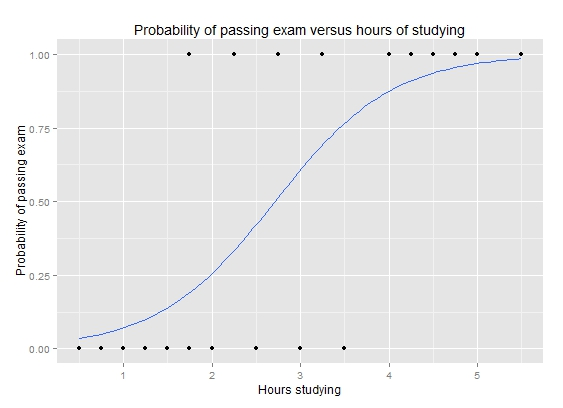
\includegraphics[width=\textwidth]{figures/regression/Exam_pass_logistic_curve.jpeg}
\caption{
Example logistic regression curve on one input feature, by \href{https://en.wikipedia.org/wiki/File:Exam_pass_logistic_curve.jpeg}{Michaelg2015}.
}
\label{fig:logistic_regression_ex}
\end{figure}

Some assumptions of the logistic regression approach are:
$y$ is dichotomous (\ie either present or absent),
there are minimal correlations between the $x_{i}$ features (\ie no multicollinearity),
and there are no major outliers in the data.

%%%%%%%%%%%%%%%%%%%%%%%%%%%%%%%%%%%%%%%%%%%%%%%%%%%%%%%%
% \section{Gaussian Process}
% \label{Regression:GP}
% TODO
